\ESKDappendix{обязательное}{Регистр кодирующего устройства} 

\begin{figure}[h!]
  \centering
  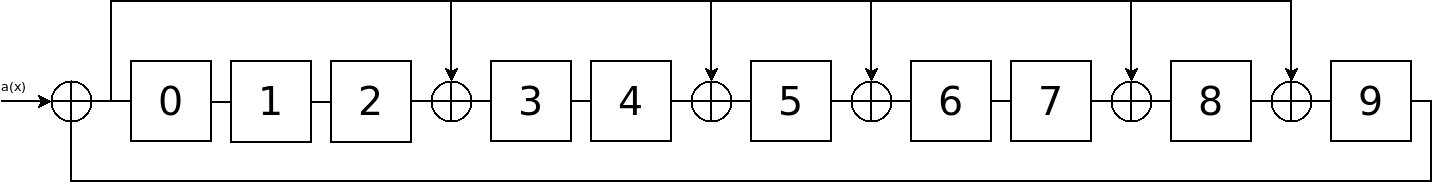
\includegraphics[width = \textwidth]{KDU}
  \caption{Схема регистра КДУ}
  \label{fig:kdu}
\end{figure}

\begin{table}[h!]
  \caption{Таблица переключений ячеек регистра}
  \begin{tabular}[h!]{|c||p{0.9cm}||p{0.9cm}||p{0.9cm}||p{0.9cm}||p{0.9cm}||p{0.9cm}||p{0.9cm}||p{0.9cm}||p{0.9cm}||p{0.9cm}|}
    \hline
    {\bf Вход} & \multicolumn{10}{c|}{{\bf Состояние ячеек}}\\\cline{2-11}
      & 0 & 1 & 2 & 3 & 4 & 5 & 6 & 7 & 8 & 9 \\ \hline \hline
    1 & 1 & 0 & 0 & 1 & 0 & 1 & 1 & 0 & 1 & 1  \\ \hline
    0 & 1 & 1 & 0 & 1 & 1 & 1 & 0 & 1 & 1 & 0  \\ \hline
    0 & 0 & 1 & 1 & 0 & 1 & 1 & 1 & 0 & 1 & 1  \\ \hline
    1 & 0 & 0 & 1 & 1 & 0 & 1 & 1 & 1 & 0 & 1  \\ \hline
    1 & 0 & 0 & 0 & 1 & 1 & 0 & 1 & 1 & 1 & 0  \\ \hline
    1 & 1 & 0 & 0 & 1 & 1 & 0 & 1 & 1 & 0 & 0  \\ \hline
    0 & 0 & 1 & 0 & 0 & 1 & 1 & 0 & 1 & 1 & 0  \\ \hline
    0 & 0 & 0 & 1 & 0 & 0 & 1 & 1 & 0 & 1 & 1  \\ \hline
    0 & 1 & 0 & 0 & 0 & 0 & 1 & 0 & 1 & 1 & 0  \\ \hline
    0 & 0 & 1 & 0 & 0 & 0 & 0 & 1 & 0 & 1 & 1  \\ \hline
    1 & 0 & 0 & 1 & 0 & 0 & 0 & 0 & 1 & 0 & 1  \\ \hline
    1 & 0 & 0 & 0 & 1 & 0 & 0 & 0 & 0 & 1 & 0  \\ \hline
    1 & 1 & 0 & 0 & 1 & 1 & 1 & 1 & 0 & 1 & 0  \\ \hline
    1 & 1 & 1 & 0 & 1 & 1 & 0 & 0 & 1 & 1 & 0  \\ \hline
    1 & 1 & 1 & 1 & 1 & 1 & 0 & 1 & 0 & 0 & 0  \\ \hline
    0 & 0 & 1 & 1 & 1 & 1 & 1 & 0 & 1 & 0 & 0  \\ \hline
    0 & 0 & 0 & 1 & 1 & 1 & 1 & 1 & 0 & 1 & 0  \\ \hline
    0 & 0 & 0 & 0 & 1 & 1 & 1 & 1 & 1 & 0 & 1  \\ \hline
    0 & 1 & 0 & 0 & 1 & 1 & 0 & 0 & 1 & 0 & 1  \\ \hline
    0 & 1 & 1 & 0 & 1 & 1 & 0 & 1 & 0 & 0 & 1  \\ \hline
    0 & 1 & 1 & 1 & 1 & 1 & 0 & 1 & 1 & 1 & 1 \\ \hline
  \end{tabular}
  \label{tab:reg}
\end{table}

\newpage
\ESKDappendix{обязательное}{Вычисления в среде GNU Octave} 
\label{sec:octave}

Нахождение остатка от деления для полинома в
\ref{sec:hemming}-м~разделе:  

\lstinputlisting[language = Octave]{./octave/hemming_poly.txt}

Нахождение разрешённой комбинации систематического кода и остатков от
деления полиномов для \ref{sec:BCH}~раздела:

\lstinputlisting[language = Octave]{./octave/BCH_poly.txt} 

Нахождение порождающего полинома, разрешённой кодовой комбинации,
синдромов для кода БЧХ в разделе \ref{sec:Reed-Solomon}:
\label{page}
\lstinputlisting[language = Octave]{./octave/rs_poly.txt}
 \newpage

\ESKDappendix{справочное}{Программа для нахождения таблицы состояний
регистра}
\lstinputlisting[language = C++]{./octave/KDU.cpp}

%%% Local Variables: 
%%% mode: plain-tex
%%% TeX-master: "../TermWork_PDS"
%%% End: 
